\documentclass{beamer}
\usepackage[ngerman]{babel}
\usepackage{beamerthemeshadow}
\useinnertheme{circles}
\usepackage [latin1]{inputenc}
\usepackage [T1]{fontenc}
\usepackage{ae}
\usepackage{lmodern}
\usetheme{Copenhagen}
\usecolortheme{seahorse}
\definecolor{codecolor}{gray}{0.73}
\beamersetuncovermixins{\opaqueness<1>{25}}{\opaqueness<2->{15}}
\beamertemplatenavigationsymbolsempty
\usepackage[savemem]{listings}
\lstdefinestyle{outline}{
numbers=left,
captionpos=b,
stepnumber=1,
numbersep=5pt,
numberstyle=\tiny,
breaklines=true,
breakautoindent=true,
postbreak=\space,
tabsize=5,
basicstyle=\ttfamily\footnotesize,
showspaces=false,
showstringspaces=false,
extendedchars=true,
backgroundcolor=\color{codecolor},
%caption=\lstname
}    
\begin{document}

\title{OpenSuSE - KIWI Image System}
\author{Marcus Sch�fer}
\date{\today} 

%==========================================
% Slide 0
%------------------------------------------
\frame{\titlepage} 

%==========================================
% Slide 1
%------------------------------------------
\begin{frame}
\frametitle{Inhaltsverzeichnis}
	\tableofcontents
\end{frame}

%==========================================
% Slide 2
%------------------------------------------
\section{Einf�hrung}
\begin{frame}
\frametitle{Was ist KIWI ?}
	\begin{itemize}
		\item Service zur Erstellung von OS Images
		\item Unterst�tzung bei der Aktivierung von OS Images
		\item Unterst�tzung von Virtualisierungssystemen (Xen)
		\item Distributionsunabh�ngig
	\end{itemize}
\end{frame}

%==========================================
% Slide 3
%------------------------------------------
\subsection{Architektur}
\begin{frame}
\frametitle{Architektur}
	\begin{figure}[h]
	\centering
	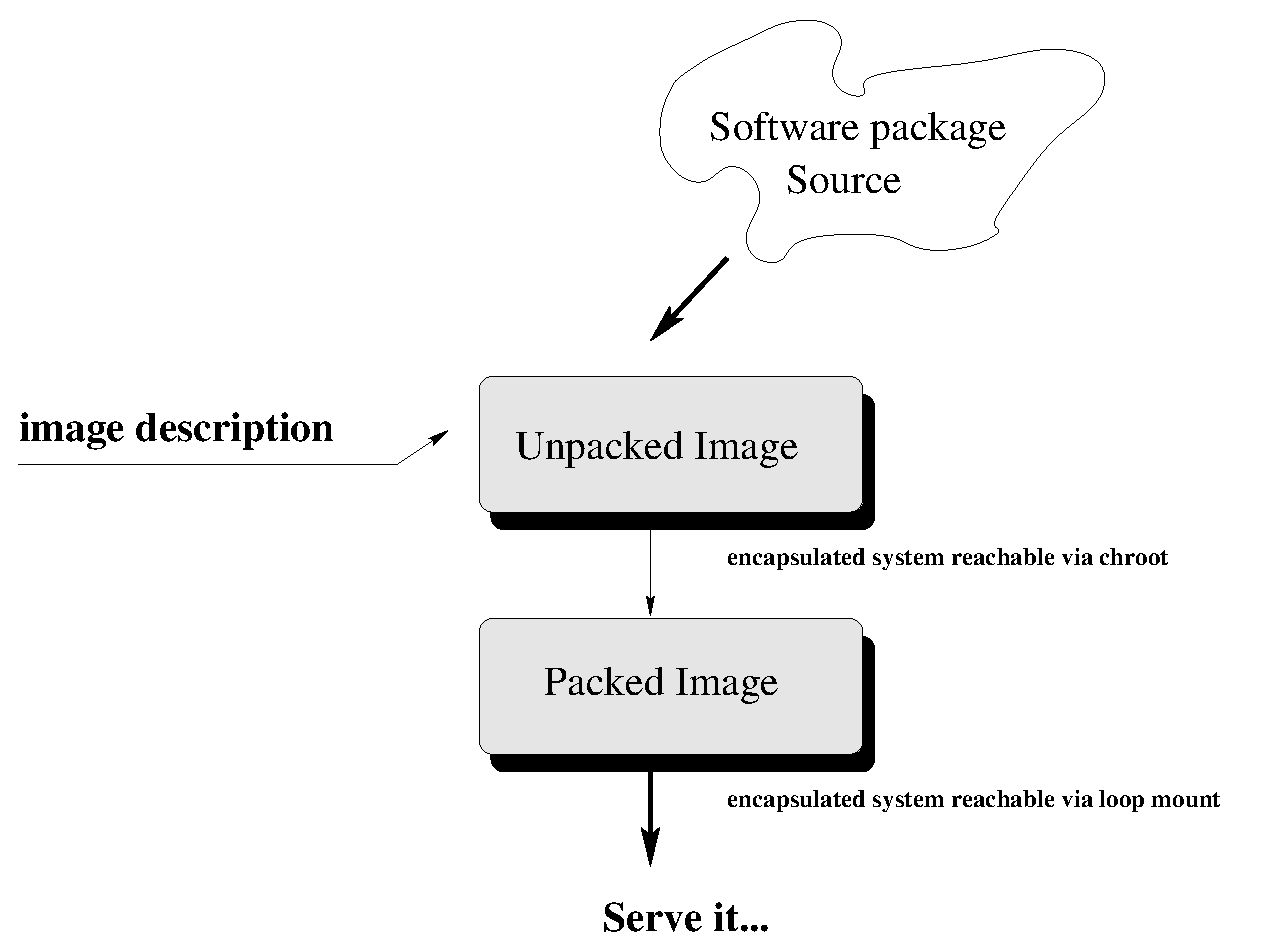
\includegraphics[scale=0.4]{../pictures/intro.eps}
	\end{figure}
\end{frame}

%==========================================
% Slide 4
%------------------------------------------
\section{Grunds�tzliches}
\begin{frame}
\frametitle{Ein Image System}
	\begin{itemize}
		\item erfordert Kenntnisse �ber das Betriebssystem. Die
              notwendigen Informationen wie das Image zu erstellen ist
              m�ssen durch den Benutzer beschrieben werden.
		\item teilt sich auf in einen Prozess- und Managementanteil.
              KIWI implementiert den Prozessteil f�r
              ein Imagesystem da der Managementanteil sehr
              von dem jeweiligen Einsatzgebiet abh�ngt
	\end{itemize}
\end{frame}


%==========================================
% Slide 5
%------------------------------------------
\subsection{Image Beschreibung}
\begin{frame}
\frametitle{Image Beschreibungs Verzeichnis: \textit{buildhost-suse-10.1/}}
	\begin{itemize}
		\item VERSION
		\item config.xml
	\end{itemize}
	Optionale Angaben:
	\begin{itemize}
		\item config.sh
		\item images.sh
		\item config/...
		\item root/...
	\end{itemize}
\end{frame}


%==========================================
% Slide 6
%------------------------------------------
\section{Beispiel}
\begin{frame}
\frametitle{Das OpenSuSE buildhost image}
	\begin{itemize}
		\item Stellt das Basisbetriebssystem zur Verf�gung um innerhalb des
              OpenSuSE Buildservice als buildhost zum Bauen von Paketen zu
              funktionieren
		\item Soll Virtualisierungssupport enthalten
		\item Alle buildhosts werden innerhalb ihres Netzes automatisch
              registriert und bespielt. Zu diesem Zweck wird ein
              netboot Image zur Verf�gung gestellt.
	\end{itemize}

	\vspace*{1cm}
	\textit{Let's go... :-)}
\end{frame}

\end{document}
